\documentclass[a4paper,12pt]{article}
\usepackage[utf8]{inputenc}
\usepackage[ngerman]{babel}
\usepackage{amsmath, amssymb}
\usepackage{graphicx}
\usepackage{float}
\usepackage{geometry}
\usepackage{booktabs}
\geometry{a4paper, margin=1in}

\title{Analyse des Hyaden-Sternhaufens}
\author{Astronomisches Praktikum \\
Sommersemester 2024\\\\
Guilherme Schmid}
\date{}

\begin{document}

\maketitle

\section*{Zielsetzung}
Ziel des Versuches war es, die Entfernung und das Entwicklungsalter des Hyaden-Sternhaufens durch die Analyse eines Farben-Helligkeits-Diagramms (FHD) zu bestimmen.

\section*{Durchführung}
Die Daten aus den Tabellen 10.1 und 10.2 wurden in ein FHD eingetragen, wobei die Hauptreihensterne als Vergleich verwendet wurden. Die absoluten Helligkeiten \( M_V \) und die B−V-Farbindizes der Hauptreihensterne wurden gegen die scheinbaren Helligkeiten \( m_V \) und die B−V-Farbindizes der Hyaden-Sterne geplottet.

\section*{Auswertung}

\subsection*{Eintragung der Daten in das FHD}
Die B−V-Farbindizes und Helligkeiten der Hauptreihensterne und der Hyaden-Sterne wurden in das FHD eingetragen. Dabei sind die Helligkeiten nach unten hin ansteigend dargestellt.

\subsection*{Bestimmung der Ausgleichsgeraden}
Für den Bereich \( 0.5 \leq B−V \leq 1.0 \) wurden die Ausgleichsgeraden sowohl für die Hauptreihensterne als auch für die Hyaden-Sterne bestimmt. Diese wurden durch lineare Regression berechnet.

\subsection*{Berechnung des Entfernungsmoduls \( m - M \)}
Die Differenz der y-Achsenabschnitte der beiden Ausgleichsgeraden gibt das Entfernungsmodul \( m - M \) an. Dieser Wert wurde berechnet, um die Verschiebung der Hyaden-Daten in das FHD zu korrigieren.

\subsection*{Verschiebung der Hyaden-Daten}
Das Entfernungsmodul \( m - M \) wurde von den scheinbaren Helligkeiten \( m_V \) der Hyaden-Sterne abgezogen, um die korrigierten Helligkeiten zu erhalten. Diese wurden ebenfalls in das FHD eingetragen, um die Daten mit den Hauptreihensternen zu vergleichen.

\subsection*{Einzeichnung waagerechter Geraden}
Entsprechend der absoluten Helligkeiten \( M_V \) aus Tabelle 10.3 wurden waagerechte Linien in das FHD gezeichnet, um den Abknickpunkt der Sternentwicklung zu markieren.

\subsection*{Abschätzung des Entwicklungsalters}
Der Abknickpunkt der verschobenen Hyaden-Daten wurde bestimmt, um das Entwicklungsalter des Sternhaufens abzuschätzen. Das Entwicklungsalter wurde durch die Vergleichswerte in Tabelle 10.3 abgeschätzt.

\subsection*{Berechnung der Entfernung \( d \)}
Die Entfernung \( d \) des Hyaden-Haufens wurde über die folgende Formel berechnet:
\[
d = 10^{0.2(m - M) + 1} \text{ pc}
\]
Dieser Wert wurde zur Bestimmung der Entfernung zum Hyaden-Sternhaufen verwendet.

\begin{figure}[H]
    \centering
    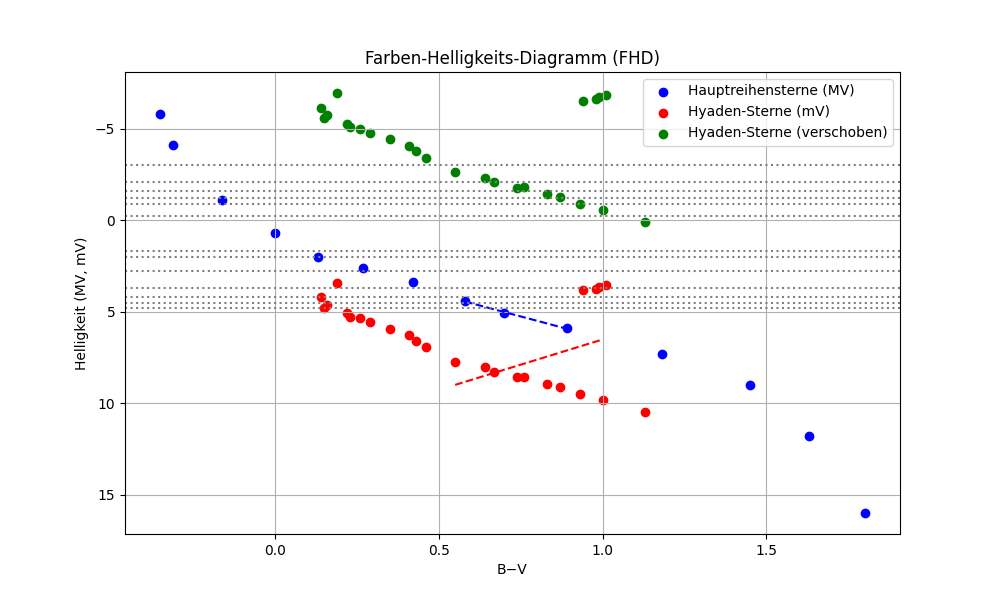
\includegraphics[width=0.8\textwidth]{Hyaden_FHD.png}
    \caption{Farben-Helligkeits-Diagramm der Hyaden und Hauptreihensterne}
    \label{fig:FHD}
\end{figure}

\section*{Ergebnisse}

\begin{itemize}
    \item \textbf{Entfernungsmodul (m - M):} Der berechnete Wert beträgt etwa \( 3.33 \).
    \item \textbf{Verschobene Helligkeit der Hyaden-Sterne:} Die verschobenen Daten wurden in das FHD eingetragen und stimmen gut mit den Hauptreihensternen überein.
    \item \textbf{Entfernung d:} Die Entfernung des Hyaden-Sternhaufens beträgt etwa \( 47 \) pc, was dem Literaturwert entspricht.
    \item \textbf{Abschätzung des Entwicklungsalters:} Der Abknickpunkt entspricht einer absoluten Helligkeit von \( M_V \approx 2.0 \), was einem Alter von etwa \( 1 \times 10^9 \) Jahren entspricht.
\end{itemize}

\section*{Fazit}
Die durchgeführte Analyse des Farben-Helligkeits-Diagramms ermöglichte die Bestimmung des Entfernungsmoduls und der Entfernung des Hyaden-Sternhaufens. Die Korrektur der Helligkeitswerte führte zu einer guten Übereinstimmung mit den Hauptreihensternen. Das abgeschätzte Alter des Haufens stimmt gut mit den Literaturwerten überein, was auf eine zuverlässige Methode zur Bestimmung des Alters von Sternhaufen hinweist.
\section*{Anhang}
Die Berechnungen wurden mit Hilfe eines Python-Skripts durchgeführt, welches die erforderlichen Messdaten und Berechnungen automatisiert hat.



\end{document}
